%%% BioMarkerScreening.tex --- 
%% Version: $Id: BioMarkerScreening.tex,v 0.0 2012/05/08 02:44:59 tangboyun Exp$
%% Copyright : (c) 2012 Boyun Tang
%% License : GPL3
\documentclass{standalone}
\usepackage{tikz}
\usetikzlibrary{mindmap,shadows,shapes.arrows,shapes.geometric,shapes.misc,matrix,arrows,positioning,calc,decorations.pathreplacing,petri}
\usepackage{graphicx}
\usepackage{times}
\usepackage{xcolor}
\begin{document}
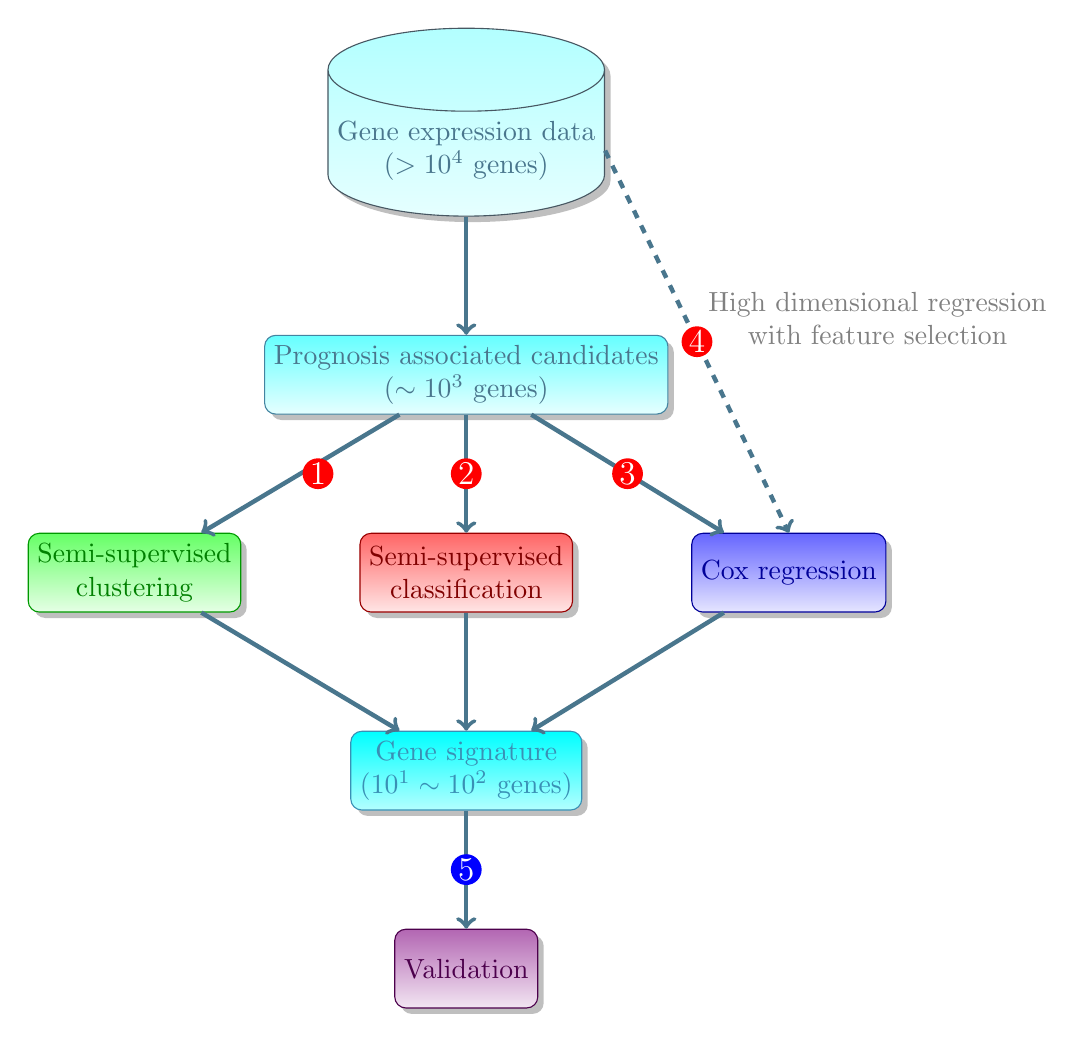
\begin{tikzpicture}[
  every node/.style={minimum height=1cm,align=center},%
  d/.style={rounded corners},%
  cl/.style={cylinder,aspect=.3,shape border rotate=90,},%
  e/.style={->,ultra thick,rounded corners,cyan!50!black},%
  t/.style={midway,token,fill=red,font=\large},%
  ]

  \node (data) [cl,
  top color= cyan!30,bottom color= cyan!10,draw=cyan!30!black,
  text=cyan!50!black,
  drop shadow,
  ] {Gene expression data\\($> 10^4$ genes)};

  \node (candidate) [d,
  below =of data,drop shadow,
  top color= cyan!60,bottom color= cyan!10,draw=cyan!60!black,
  text=cyan!50!black,
  yshift = -0.5cm,
  ] {Prognosis associated candidates\\($\sim 10^3$ genes)};

  \node (classification) [d,
  below =of candidate,drop shadow,
  top color= red!60,bottom color= red!10,draw=red!60!black,
  text=red!50!black,
  yshift = -0.5cm,
  ] {Semi-supervised\\classification};

  \node (clustering) [d,
  left = of classification,drop shadow,
  top color= green!60,bottom color= green!10,draw=green!60!black,
  text=green!50!black,
  xshift=-0.5cm,
  ] {Semi-supervised\\clustering};

  \node (regression) [d,
  right = of classification,drop shadow,
  top color= blue!60,bottom color= blue!10,draw=blue!60!black,
  text=blue!60!black,
  xshift=0.5cm,
  ] {Cox regression};

  \node (signature) [d,
  below = of classification,drop shadow,
  top color= cyan,bottom color= cyan!30,draw=cyan!70!black,
  text=cyan!70!black,
  yshift=-0.5cm,
  ] {Gene signature\\($10^1\sim 10^2$ genes)};
 
  \node (validation) [d,
  below = of signature,drop shadow,
  top color= violet!60,bottom color= violet!10,draw=violet!60!black,
  text=violet!60!black,
  yshift=-0.5cm,
  ] {Validation};

  \draw [e] (data) -- (candidate);
  \draw [e] (candidate) -- (classification) node [t] {2};
  \draw [e] (candidate) -- (clustering) node [t,right] {1};
  \draw [e] (candidate) -- (regression) node [t] {3};
  \draw [e] (classification) -- (signature);
  \draw [e] (clustering) -- (signature);
  \draw [e] (regression) -- (signature);
  \draw [e] (signature) -- (validation) node [t,fill=blue] {5};

  \draw [e,dashed] (data.east) -- (regression.north) 
  node [midway,right,yshift=0.3cm,text=gray] 
  {High dimensional regression\\with feature selection};

  \path (data.east) -- (regression.north) node [t] {4};
\end{tikzpicture}  

\end{document}


%%% Local Variables: 
%%% TeX-master: t
%%% End: 
